\documentclass[12pt, a4paper, oneside]{book} 
\usepackage{svn-multi}
\usepackage{makecell}

\tolerance=10000
\vfuzz=8pt

\usepackage{lipsum}

\usepackage{silence}
\WarningFilter{hyperref}{Invalid value `0'}
\WarningFilter{latex}{Some font shapes were not available, defaults substituted.}
\usepackage{amsmath}

\svnid{$Id$}
\usepackage{prelim2e}
\renewcommand{\PrelimWords}{Draft Copy \svnkw{Id}}

%%\newcommand*{\mysvnrev}{\svnrev}
\usepackage[hyperindex=true,
			bookmarks=true,
            pdftitle={}, pdfauthor={Olivia Walters},
            colorlinks=false,
            pdfborder=0,
            pagebackref=false,
            citecolor=blue,
            plainpages=false,
            pdfpagelabels,
            pagebackref=true,
            hyperfootnotes=false]{hyperref}
\usepackage[all]{hypcap}
\usepackage[palatino]{anuthesis}
\usepackage{afterpage}
\usepackage{graphicx}
\usepackage{thesis}
\usepackage{textcomp}
\usepackage[square]{natbib}
\usepackage[normalem]{ulem}
\usepackage[table]{xcolor}
\usepackage{makeidx}
\usepackage{cleveref}
\usepackage[centerlast]{caption2}
\usepackage{float}
\urlstyle{sf}
\renewcommand{\sfdefault}{cmr}
\usepackage[T1]{fontenc}
\usepackage[scaled]{beramono}

\usepackage{multirow}

\graphicspath{{../../Resources/Figures}}


\renewcommand*{\backref}[1]{}
\renewcommand*{\backrefalt}[4]{
  \ifcase #1 %
    %
  \or
    (cited on page #2)%
  \else
    (cited on pages #2)%
  \fi
}




%      $Id: macros.tex 506 2009-10-05 16:57:07Z daniel $    

\usepackage{booktabs}
\usepackage{relsize}
\usepackage{xspace}
\usepackage{subfigure}
\usepackage{listings}
\lstloadlanguages{java}
\DeclareGraphicsRule{*}{pdf}{*}{}
\newcommand{\otoprule}{\midrule[\heavyrulewidth]}
\newcommand{\pldi}{ACM Programming Language Design and Implementation (PLDI)}
\newcommand{\taco}{ACM Transactions on Architecture and Code Optimization (TACO)}
\newcommand{\lctes}{ACM Languages, Compiler, and Tool Support for Embedded Systems (LCTES)}
\newcommand{\popl}{ACM Principles of Programming Languages (POPL)}
\newcommand{\ecoop}{European Conference for Object-Oriented Programming (ECOOP)}
\newcommand{\asplos}{ACM Architectural Support for Programming Languages and Operating Systems (ASPLOS)}
\newcommand{\sigmetrics}{ACM Measurement and Modeling of Computer Systems (SIGMETRICS)}
\newcommand{\oopsla}{ACM Object-Oriented Programming, Systems, Languages, and Applications (OOPSLA)}
\newcommand{\ismm}{International Symposium on Memory Management (ISMM)}
\newcommand{\veee}{ACM/USENIX Virtual Execution Environments (VEE)}
\newcommand{\micro}{ACM/IEEE International Symposium on Microarchitecture}
\newcommand{\isca}{ACM/IEEE International Symposium on Computer Architecture (ISCA)}
\newcommand{\icse}{International Conference  on Software Engineering (ICSE)}
\newcommand{\pact}{Parallel Architectures and Compilation Techniques (PACT)}
\newcommand{\casess}{ACM Compilers, Architectures, and Synthesis for Embedded Systems (CASES)}

\definecolor{tableheadcolor}{rgb}{0.8,0.8,1.0}
%\definecolor{tablealtcolor}{rgb}{0.9,0.9,1.0}
\definecolor{tablealtcolor}{rgb}{0.9,0.9,0.95}


\definecolor{todocolor}{rgb}{0.8,0.8,1.0}
\definecolor{fixcolor}{rgb}{1,0.8,0.8}
\definecolor{commentcolor}{rgb}{0.8,1.0,0.8}


\newcommand{\listingfigure}[3]{
\begin{figure}[ht!]
  \begin{center}
    \begin{minipage}[t]{\textwidth-4cm}
      \lstinputlisting{#1}
    \end{minipage}
  \end{center}
  \caption{#3}#2
\end{figure}}

\newcommand{\includeabchart}[5]{
\begin{figure}[ht!]
\begin{center}
\newcommand{\atitle}{#4}
\newcommand{\btitle}{#5}
\input{charts/#1.tex}
\end{center}
\caption{#3}#2
\end{figure}}

\newcommand{\placeholderfigure}[2]{
\begin{figure}[ht!]
  \begin{center}
    \resizebox{\textwidth-2cm}{0.7\textwidth-1.4cm}{todo}
  \end{center}
  \caption{#2}#1
\end{figure}}

\newcommand{\singlegraphfigure}[3]{
\begin{figure}[ht!]
  \begin{center}
    \includegraphics[width=\textwidth-2cm]{#1}
  \end{center}
  \caption{#3}#2
\end{figure}}

\usepackage[color=todocolor, colorinlistoftodos]{todonotes}

%\newcommand{\notinpart}{%
% \def\toclevel@chapter{-1}\def\toclevel@section{0}\def\toclevel@subsection{1}} \newcommand{\inpart}{
% \def\toclevel@chapter{0}\def\toclevel@section{1}\def\toclevel@subsection{2}}


%
% Stuff for pretty printing the source code using listings.sty
%


%% set Java as the default language
\lstset{
  numbers=left,
  numberstyle=\tiny,
  stepnumber=1,
  numbersep=2em,
  language=java,                         % the language
  basicstyle=\footnotesize\ttfamily,     % the basic font family to use
  commentstyle=\itshape,                 % the font for comments
  stringstyle=\ttfamily,
%  morekeywords={@Intrinsic, @Unboxed, @RawStorage}
}
%\lstset{language=java}

\newcommand{\textjava}[1]{{\lstset{basicstyle=\ttfamily}\lstinline@#1@}}
\newcommand{\textjavafn}[1]{{\lstset{basicstyle=\footnotesize\ttfamily}\lstinline@#1@}}
%\usepackage{lstasm}
\usepackage{setspace}
\usepackage{ifthen}
%\usepackage{color}
%\usepackage{smallheadings}

\long\def\sfootnote[#1]#2{\begingroup%
\def\thefootnote{\fnsymbol{footnote}}\footnote[#1]{#2}\endgroup}
%
% code
%

\newcommand{\address}{\textjava{Address}\xspace}
\newcommand{\ubregion}{\textjava{unbump-region()}\xspace}
\newcommand{\word}{\textjava{Word}\xspace}
\newcommand{\freeme}{\textjava{free()}\xspace}
\newcommand{\freemeunbump}{\textjava{unbump()}\xspace}
\newcommand{\freemeunbumpregion}{\textjava{unbump-region()}\xspace}
\newcommand{\freemeunreserve}{\textjava{unreserve()}\xspace}

%
% abbreviations
%


\newcommand{\eg}{e.g., }
\newcommand{\ie}{i.e., }

\newcommand{\GenMS}{\emph{GenMS}\xspace}
\newcommand{\GenImmix}{\emph{GenIX}\xspace}
\newcommand{\mmtk}{MMTk\xspace}
\newcommand{\jikes}{Jikes RVM\xspace} 
\newcommand{\jikesrvm}{\jikes} 
\newcommand{\jala}{Jalape\~{n}o\xspace} 
\newcommand{\jalapeno}{Jalape\~{n}o\xspace} 

\newcommand{\dacapo}{\textsf{DaCapo}\xspace}
\newcommand{\specjvm}{\textsf{SPECjvm98}\xspace}
\newcommand{\cattrack}{\textsf{cattrack}\xspace}
\newcommand{\spec}{\textsf{SPEC}\xspace}

\newcommand{\nurserytype}[1]{{\fontfamily{cmss}\selectfont \textsl{#1}}}
\newcommand{\alloc}{\nurserytype{allocate}\xspace}
\newcommand{\collect}{\nurserytype{collect}\xspace}
\newcommand{\redirect}{\nurserytype{redirect}\xspace}

\newcommand{\bmtype}[1]{{\textsf{#1}}}

\newcommand{\jbb}{\bmtype{jbb2000}\xspace}
\newcommand{\psjbb}{\bmtype{pjbb2005}\xspace}
\newcommand{\pjbb}{\bmtype{pjbb2005}\xspace}
\newcommand{\specjbb}{\bmtype{SPECjbb2005}\xspace}
\newcommand{\jess}{\bmtype{jess}\xspace}
\newcommand{\raytrace}{\bmtype{raytrace}\xspace}
\newcommand{\db}{\bmtype{db}\xspace}
\newcommand{\javac}{\bmtype{javac}\xspace}
\newcommand{\jack}{\bmtype{jack}\xspace}
\newcommand{\compress}{\bmtype{compress}\xspace}
\newcommand{\mpegaudio}{\bmtype{mpegaudio}\xspace}
\newcommand{\mtrt}{\bmtype{mtrt}\xspace}
\newcommand{\antlr}{\bmtype{antlr}\xspace}
\newcommand{\bloat}{\bmtype{bloat}\xspace}
\newcommand{\chart}{\bmtype{chart}\xspace}
\newcommand{\eclipse}{\bmtype{eclipse}\xspace}
\newcommand{\fop}{\bmtype{fop}\xspace}
\newcommand{\hsqldb}{\bmtype{hsqldb}\xspace}
\newcommand{\jython}{\bmtype{jython}\xspace}
\newcommand{\luindex}{\bmtype{luindex}\xspace}
\newcommand{\lusearch}{\bmtype{lusearch}\xspace}
\newcommand{\Lusearch}{\bmtype{Lusearch}\xspace}
\newcommand{\pmd}{\bmtype{pmd}\xspace}
\newcommand{\ps}{\bmtype{ps}\xspace}
\newcommand{\SPECjbb}{\bmtype{SPECjbb}\xspace}
\newcommand{\xalan}{\bmtype{xalan}\xspace}
\newcommand{\sunflow}{\bmtype{sunflow}\xspace}
\newcommand{\Sunflow}{\bmtype{Sunflow}\xspace}
\newcommand{\avrora}{\bmtype{avrora}\xspace}
\newcommand{\core}{Core2 Quad\xspace}
\newcommand{\corelong}{Intel Core2 Quad Q6600\xspace}
\newcommand{\phenom}{Phenom II\xspace}
\newcommand{\phenomlong}{AMD Phenom II X6 1055T\xspace}
\newcommand{\sandy}{i7-2600\xspace}
\newcommand{\sandylong}{Intel Core i7-2600\xspace}



\newcommand{\ghostscript}{\bmtype{ghostscript}\xspace}

\newcommand{\doi}[1]{\href{http://dx.doi.org/#1}{\nolinkurl{doi:#1}}}
%
% misc
%
\newcommand{\fix}[1]{\todo[color=fixcolor]{#1}}
\newcommand{\comment}[1]{\todo[color=commentcolor]{#1}}
\newcommand{\ifix}[1]{\todo[inline,color=fixcolor]{#1}}
\newcommand{\icomment}[1]{\todo[inline,color=commentcolor]{#1}}
\newcommand{\itodo}[1]{\todo[inline]{#1}}
\newcommand{\ignore}[1]{}
\newcommand{\mccenter}[1]{\multicolumn{1}{c|}{#1}}

%
% figure spacing
%
%\clubpenalty 10000
%\widowpenalty 10000
%\def\topfraction{0.9}
%\def\bottomfraction{0.9}
%\def\textfraction{0.1}
%\renewcommand{\singlespacing}{\renewcommand{\baselinestretch}{1.00}\small\normalsize}
%\renewcommand{\doublespacing}{\renewcommand{\baselinestretch}{1.5}\small\normalsize}
%\newcommand{\tight}{\renewcommand{\baselinestretch}{1.28}\small\normalsize}
%\renewcommand{\subfigbottomskip}{0.25ex}
%\renewcommand{\subfigcapskip}{0ex}
%\renewcommand{\subfigcapskip}{-1ex}
%\newcommand{\subfigshrink}{-0.75ex}
%\newcommand{\subfigcapspace}{2ex}

%\newcommand{\subwidth}[0]{.32\textwidth}


%
% margins
%
%\topmargin -.5truein
%\textheight 9truein
%\oddsidemargin .25truein
%\evensidemargin .25truein
%\textwidth 6truein


%
% crossreferencing footnotes
%
%\newcommand{\fnref}[1]{~(\ref{#1})}
%\newcommand{\onecolparbox}{3.1in}


%\newcommand{\textjava}[1]{{\lstset{language=java,basicstyle=\footnotesize\ttfamily}\lstinline@#1@}}
%\newcommand{\textasm}[1]{{\lstset{language=asm,basicstyle=\footnotesize\ttfamily}\lstinline@#1@}}

%%
%% Change the sections etc.
%%
%\makeatletter
%\parskip=0pt
%\renewcommand\section{\@startsection{section}{1}{\z@}%
%                                   {-2.5ex}% beforeskip
%%                                   {1ex}% afterskip
%                                   {\large \bfseries \raggedright}}
% \renewcommand\subsection{\@startsection{subsection}{2}{\z@}%
%                                     {-2ex\@plus -1ex \@minus -.2ex}%
%                                      {.5ex \@plus .2ex}%
%                                      {\normalsize \bfseries \raggedright}}
% \renewcommand\subsubsection{\@startsection{subsubsection}{3}{\z@}%
%                                      {-2ex\@plus -1ex \@minus -.2ex}%
%                                      {1ex \@plus .2ex}%
%                                      {\normalfont\fontsize{11pt}{12pt}\selectfont\itshape}}
%\renewcommand{\thesubsubsection}{\thesubsection.\arabic{subsubsection}}

%\renewcommand\paragraph{\@startsection{paragraph}{4}{\z@}% 
%  {.5em}%
%  {-1em}%
%  {\normalfont\normalsize\bfseries\parskip=0pt}}
%\setlength\partopsep{0\p@}
%\setlength\parskip{0\p@ \@plus \p@}

%\makeatother
%\parindent=9pt





%%% Local Variables: 
%%% mode: latex
%%% TeX-master: "doa"
%%% End:
            
%%%%%%%%%%%%%%%%%%%%%%%%%%%%%%%%%%%%%%%%%%%%%%%%%%%%%%%%%%%%%%%%%%%%%%%
%% Preamble
\title{Magnetic fields in circumgalactic high velocity clouds}
\author{Olivia Walters}
\date{\today}

\renewcommand{\thepage}{\roman{page}}

\makeindex
\begin{document}

\hbadness=10000

%\doparttoc
%%%%%%%%%%%%%%%%%%%%%%%%%%%%%%%%%%%%%%%%%%%%%%%%%%%%%%%%%%%%%%%%%%%%%%%
%% Title page
\pagestyle{empty}
\thispagestyle{empty}
%% anuthesis.sty Copyright (C) 1996, 1997 Steve Blackburn
%% Department of Computer Science, Australian National University
%%

\begin{titlepage}
  \enlargethispage{2cm}
  \begin{center}
    \makeatletter
    \Huge\textbf{\@title} \\[.4cm]
    \Huge\textbf{\thesisqualifier} \\[2.5cm]
    \huge\textbf{\@author} \\[9cm]
    \makeatother
%%   \LARGE A thesis submitted for the degree of \\
%%    Master of Philosophy at \\
%%    The Australian National University \\[2cm]
    \LARGE A thesis submitted for the degree of \\
    Test Github integration \\
    The Australian National University \\[2cm]
    \thismonth
  \end{center}
\end{titlepage}


%%%%%%%%%%%%%%%%%%%%%%%%%%%%%%%%%%%%%%%%%%%%%%%%%%%%%%%%%%%%%%%%%%%%%%%
%% Here begin the preliminaries
\vspace*{14cm}
\begin{center}
  \makeatletter
  \copyright\ \@author{} 2024
  \makeatother
\end{center}
\noindent
\begin{center}
  \footnotesize{~} %\aboutthesis
\end{center}
\noindent

\newpage

\addcontentsline{toc}{chapter}{Statement of Originality}

\vspace*{7cm}
\begin{center}
  Except where otherwise indicated, this thesis is my own original
  work.
\end{center}

\vspace*{4cm}

\hspace{8cm}\makeatletter\@author\makeatother\par
\hspace{8cm}\today


%%%%%%%%%%%%%%%%%%%%%%%%%%%%%%%%%%%%%%%%%%%%%%%%%%%%%%%%%%%%%%%%%%%%%%%
%% Dedication
%\cleardoublepage
%\pagestyle{empty}
%\vspace*{7cm}
\begin{center}
  To my grandmother, Hilda Filipovic, for being a very important person in my life, and a rock on which I relied on in the process of completeing my honours year.
\end{center}

\vspace*{4cm}

%%%%%%%%%%%%%%%%%%%%%%%%%%%%%%%%%%%%%%%%%%%%%%%%%%%%%%%%%%%%%%%%%%%%%%%
%% Acknowledgements
\cleardoublepage
\pagestyle{empty}
\chapter*{Acknowledgments}
\addcontentsline{toc}{chapter}{Acknowledgments}


I would like to thank my primary and secondary supervisors, Dr. Craig Anderson and Prof. Naomi-McClure Griffiths for being the main body of support, data, and ideas when writing this thesis. I would also like to acknowledge Prof. Brian Gaensler and Dr. Lyla Jung for providing further aid in the process of analysis, and their support in regards to POSSUM itself. The ASKAP POSSUM team more broadly has come as a great aid and source of community during the production of this thesis.

Fellow radio astronomer Callum Lynn has also been a great source of advice and help in constructing this thesis for a more general astronomical audience, along with his guidance about the honours and PhD process.

The ANU SSN Consultancy Group was a crucial part in the validation of the statistical techniques listed in this paper, including the suggestion to use the Weighted ANOVA and Tukey HSD test.

I would also like to thank my grandmother, Hilda Filipovic, for being a very important person in my life, and a rock on which I relied on in the process of completeing my honours year.

%%%%%%%%%%%%%%%%%%%%%%%%%%%%%%%%%%%%%%%%%%%%%%%%%%%%%%%%%%%%%%%%%%%%%%%
%% Abstract
\cleardoublepage
\pagestyle{headings}
\chapter*{Abstract}
\addcontentsline{toc}{chapter}{Abstract}
\vspace{-1em}

\lipsum[1]

%%% Local Variables: 
%%% mode: latex
%%% TeX-master: "paper"
%%% End: 

%%%%%%%%%%%%%%%%%%%%%%%%%%%%%%%%%%%%%%%%%%%%%%%%%%%%%%%%%%%%%%%%%%%%%%%
%% Table of contents
\cleardoublepage
\pagestyle{headings}
\markboth{Contents}{Contents}
\tableofcontents
\listoffigures
\listoftables

%%%%%%%%%%%%%%%%%%%%%%%%%%%%%%%%%%%%%%%%%%%%%%%%%%%%%%%%%%%%%%%%%%%%%%
%% Here begins the main text
\mainmatter

%% Introduction
\chapter{Introduction}
\label{cha:introduction}

The question of how gas is accreted into galaxies fuelling star-formation is a puzzle that has perplexed astronomers for decades \citep{ID28,ID23}. Due to the complexities in the structures of star-forming galaxies, there are many factors involved in the process of, and potential sources of accretion. What astronomers do know, at least, is that star-forming galaxies require a continuous supply of fresh gas to continue their star formation \citep{ID28,ID23, ID19}.


Due to observational constraints, astronomers are required to attempt to answer this question by examining the behaviours of our own Milky Way and Local Group environment, assuming the Milky Way is typical of a star-forming galaxy.


A major factor to consider when answering this question is where fresh pristine gas comes from, and by what mechanism it takes to enter the disks of star-forming galaxies \citep{ID8, ID28, ID49}. High Velocity Clouds (HVCs) have been a suggested mechanism for Galactic gas accretion and this report aims to evaluate the viability of this suggestion \citep{ID3,ID19}. 


\section{High Velocity Clouds}
\label{sec:hvcs}

HVCs are clouds of gas found in the Milky Way's Circumgalactic Medium (CGM) and Galactic halo. They have a high peculiar velocity relative to the Galactic Standard of Rest (GSR), typically 70-90 $\mathrm{km s^{-1}}$ \citep{ID7, ID8}. As will be shown in section \ref{ssec:draping}, this increased speed, and its interaction with halo magnetic fields, is hypothesized to allow the HVC to survive as it travels through the CGM and halo so it can reach the Galactic disk and Interstellar Medium (ISM) of the Milky Way.


There are a few hypothesises as to where HVCs originate. \cite{ID19} suggests that HVCs originate from the Intergalactic Medium (IGM) surrounding the local group. However, there is also a belief that some HVCs likely 'tore off' from satellites like the Magellanic Clouds, due to the presence of their own dark matter subhaloes, and the existence of HVCs in the Magellanic Stream and Leading Arm \citep{ID27, ID2}. Recent simulations from TNG50 have indicated that HVCs mainly have their origins in the warm-hot CGM, formed through cooling from thermal instabilities \citep{ID74}.


HVCs typically have a neutral mass gas content of $10^5 - 3\times10^5 M_{\odot}$ \citep{ID19}. They are generally shaped like comets, with a primary bulb that is approximately 0.5-25 kpc in diameter - a value that is highly dependent on distance to the Galactic midplane, which can range from approx. 2 kpc - 15 Mpc \citep{ID19, ID13}. Furthermore, HVCs have tail-like structures that account for one eighth the baryonic mass of the HVC \citep{ID13}. These tails leave behind long streams of gas that remain after collision with the Galactic disk \citep{ID19}. This size-distance correlation, comet-like structure, and long streaming tails suggest quite conclusively that HVCs shed large quantities of material as they make their journey to the ISM.


Figure \ref{fig:hvc_example} is from \cite{ID13}, which provides a typical example of what a HVC looks like in HI, specifically using the example of HVC125+41-207.

\begin{figure}
    \includegraphics[width=12cm]{"Konz_2002.png"}
    \centering
    \caption{From \cite{ID13}, figure 2. An example of a typical HVC shape and structure, specifically that of HVC125+41-207. The contour lines and shading indicate HI column density.}
    \label{fig:hvc_example}
\end{figure}


\section{Magnetic Fields}
\label{sec:bfields}

The primary issue facing HVCs as an explanation for gas accretion is its capacity to survive as it travels through the CGM and Galactic halo. As discussed, in section \ref{sec:hvcs}, HVCs can loose a lot of size and mass as it approaches towards the Galactic disk, with the long trails it leaves behind being evidence for ram-pressure stripping as the HVC collides with the gas present in the halo \citep{ID11, ID23, ID33}. \cite{ID25} demonstrates that without anything to counter this effect, HVCs with masses under $10^{4.5} M_{\odot}$ would completely disperse within 10 kpc of halo travel.


Additionally, HVCs are subject to Kelvin-Helmholtz (K-H) instabilities, which is triggered by the nature of the HVC being a cloud of warm gas travelling at high speeds through a medium of warm halo gas. These K-H instabilities are a significant factor that would lead a to HVC dispersing before it reaches the Galactic disk \citep{ID11, ID23, ID33}.


\subsection{Draping}
\label{ssec:draping}

The proposed solution to handle this problem is magnetic fields. The Galactic halo is magnetised to some degree \citep{ID30, ID16, ID4, ID42}. It is hypothesised that HVCs accumulate these existing magnetic fields in the Galactic halo, causing them to cloak the HVC with a shield that protects against ram pressure stripping and supresses K-H instabilities \citep{ID10, ID11, ID13, ID23, ID24, ID34}. This phenomenon is referred to as 'magnetic draping'.


There is not enough observational evidence to support the magnetic draping hypothesis. However, with recent advancements in: RM radio surveys \citep{ID52, ID71, ID1, ID3, ID6, ID18, ID43, ID44, ID45}; the analysis of ram pressure stripping \citep{ID11, ID23, ID33}; measurement and estimation of magnetic fields \citep{ID5, ID23, ID30, ID11, ID26, ID21}; and simulations of HVCs \citep{ID13, ID23, ID24, ID33, ID34} – it is now possible to attempt to observe and analyse the role of magnetic draping in HVCs observationally.


Previous and recent simulations involve reports produced by \cite{ID23, ID24, ID33} (henceforth referred to as the “\citeauthor{ID23} simulations”) that provide detailed insight onto how a magnetic draping protects HVCs from collapse, complementing earlier work by \cite{ID13, ID11}. It is shown from the \citeauthor{ID23} simulations that magnetic fields of about 0.3-1 {\textmu}G can provide stability to HVCs.


However, increasing magnetic field strength beyond a certain threshold can result in less stability; magnetic fields can accelerate the effects of Rayleigh-Taylor (R-T) instabilities and the magnetic pressure applied by the draped fields can also slow down a HVC to the point that it no longer is fast enough to sweep up these magnetic fields. From the \citeauthor{ID23} simulations, the upper threshold where these effects start increasing instability is about 1 {\textmu}G (specifically stating a maximum of approx. 3 {\textmu}G), thus HVCs should ideally have a “Goldilocks” magnetic field strength on the order of magnitude of 0.1{\textmu}G, with 1{\textmu}G being too high, and 0.01{\textmu}G being too low.


The effectiveness of magnetic draping is affected by the morphology of these fields and the physical properties of the HVC. The \citeauthor{ID23} simulations state that both the orientation of the magnetic field with respect to the direction of motion of the HVC, and where the magnetic field is located are important considerations. It is expected that HVC is not entirely covered in a magnetic field, only the part that is front facing in the direction of travel. While it is possible to draw conclusions about the survivability of a HVC from the strength of the magnetic field, modelling is required to confirm the accuracy of such conclusions \citep{ID5}. The \citeauthor{ID23} simulations also predict that metallicity can affect the HVC's survivability, via affecting phase transitions, with high-density metal-rich clouds and low-density metal-poor clouds being more unstable than HVCs of the opposite compositions.


The simulations by \cite{ID36} predict higher magnetic field strengths on the order of 1 \textmu G. It is very clear that even simulationaly, the specific strengths of magnetic fields surrounding HVCs have high uncertainty. The results of this report will still compare against the \citeauthor{ID23} simulations despite this.


\subsection{Faraday Rotation}
\label{ssec:faraday}

Magnetic fields cannot directly be imaged by a telescope. Instead, researchers can use the phenomenon of Faraday Rotation to quantify the line-of-sight magnetic field strength. Polarised radiation tends to rotate as it travels through a medium with a magnetic field present. This effect is quantified by equation \ref{eq:stokes}.

\begin{equation}
    \Delta\psi = \phi\lambda^2
    \label{eq:stokes}
\end{equation}


Where $\lambda$ is the wavelength of radiation, $\phi$ is the faraday depth and $\Delta\psi$ is the change in polarisation angle. Thus, by recording the stokes parameters of incoming light from distant radio sources, one can derive the Rotation Measure (RM) of incoming radiation, which is a statistical quantifier of Faraday Rotation and faraday depth \citep{ID1, ID14}. For the purposes of this report, rotation measure and faraday depth are treated as equivalent henceforth, despite their subtle differences.


For illustrative purposes, a schematic diagram of how Faraday Rotation is measured by telescopes on Earth with the aim of analysing HVCs are shown in figure \ref{fig:schema}.


\cite{ID1} describes the method by which this report's main source, the Polarisation Sky Survey of the Universe's Magnetism (POSSUM), obtained its RMs from radio observations. There is a direct connection between RM and line-of-sight magnetic field strength, quantified by equation \ref{eq:rm_integral} \citep{ID5, ID1, ID26, ID27, ID30}.


\begin{equation}
    \mathrm{RM} = 0.812 \int_{s_{\mathrm{observer}}}^{s_{\mathrm{source}}}{\frac{n_e(s)}{\mathrm{cm^{-2}}}\frac{B_{\parallel}}{\mu\mathrm{G}}\frac{ds}{\mathrm{pc}}} \mathrm{rad~m^{-2}}
    \label{eq:rm_integral}
\end{equation}


In which, $B_{\parallel}$ is the magnetic field strength, $\mathrm{RM}$ is the Rotation Measure, and $n_e$ is the electron density of the medium as a function of line-of-sight distance $s$. The analysis of this equation, its solutions, and the use of it in calculating the magnitude of line-of-sight magnetic fields is discussed in section \ref{cha:derivation}.


Faraday Rotation also occurs in the ISM of the Milky Way, due to the slight magnetisation of the ISM \citep{ID37, ID30, ID21}. This magnetisation is antisymmetric with galactic longnitude \citep{ID30}. Hence it is also important to remove the foreground from RM observations.


When making radio observations of RMs, a principal factor to consider is the observational signal to noise ratio and detector sensitivity. Radio sources tend to appear in the field after high exposure times as point-like sources. These point-like sources are then collated into an “RM grid” which has a particular density measured in sample points per square degree. The sensitivity of a detector and total integration time determines the number of source points observed as seen in figure \ref{fig:loi} \citep{ID59}.

\begin{figure}
    \includegraphics[width=9cm]{"Loi_2019.png"}
    \centering
    \caption{From \cite{ID59}, figure 4. A graph of the relationship between the sensitivity at 1.4 GHz (x-axis) and the average mimumum number of RM sample points per square degree (y-axis). The black points are not relevant to the report, but the purple line and equation describe the determined relationship.}
    \label{fig:loi}
\end{figure}

Signal to noise is of primary concern when measuring the effect of Faraday Rotation. At low enough signal-to-noise ratios, it is possible to encounter noise peaks which do not accurately represent the real RM \citep{ID60}. Figure \ref{fig:snr} gives a visual illustration of this phenomenon. The issue in question is that any observation of RM grids is going to dip below the signal-to-noise threshold of approx. 6, which can introduce an intrinsic scatter in collected RM grid data. Thus RM points below this threshold are ignored. However, the dataset masks out all RMs below a signal to noise of 8, which is considered conservative \citep{ID71}.

As will be discussed in section \ref{sec:ASKAP}, the POSSUM dataset is the first dataset with 30 RMs per square degree versus legacy surveys which had only 1 RM per square degree.

\begin{figure}
    \includegraphics[width=12cm]{"Macquart_2012.jpg"}
    \centering
    \caption{From \cite{ID60}, figure 1. A graph displaying the effect of observational (stokes parameters) signal-to-noise ratio the resultant faraday depth on a sample set of observations.}
    \label{fig:snr}
\end{figure}

\begin{figure}
    \includegraphics[width=10cm]{"Schematic Diagram.png"}
    \centering
    \caption{An schematic diagram illustrating how the RM of incoming radio radiation is observed, notably around HVCs. Note that the extragalactic radiation will appear as randomly distributed across the field of view.}
    \label{fig:schema}
\end{figure}

\subsection{Temperature, Chemical Properites, and Emission}
\label{sec:chem}

Due to their hypothesised origins in extragalactic gas, HVCs contain mostly hydrogen gas such as HI, which can be seen with 21 cm emission \citep{ID7, ID8, ID6}. The proportion of ionised gas in HVCs is still heavily debated. HVCs also emit H-alpha, however due to extinction effects, it is difficult to observe \citep{ID9, ID43}.

HVCs have a temperature relationship with proximity to the Galactic midplane, with an average HVC temperature of 10000 K and a range of temperatures ranging from 8000 – 12000 K \citep{ID49, ID48}. The temperature of a HVC is in the region in which atomic hydrogen transitions from neutral (HI) to ionised (HII), suggesting that HVCs may be partly ionised \citep{ID49, ID48, ID68}. This temperature relationship is dependent on their position with respect to the Galactic midplane, with HVCs closer to the midplane generally being cooler \citep{ID48}. This temperature is contrasted by the Galactic halo temperature, which varies from $\approx 10^4-10^6$ K \citep{ID19}. This is an important factor in creating K-H instabilities.


There is evidence that HVCs can contain alpha group elements. \cite{ID49, ID48} found the presence of [NII] 6583{\AA}, [SII] 6716{\AA}, and [OIII] 5007{\AA} emission lines – with a conclusion that Nitrogen abundance is 0.15-0.44 times solar abundance levels. The observation of these emission lines can help constrain the metallicity of any HVC  \citep{ID49}. Metallicity is important in both how HVCs act as fresh gas supplies for star formation. As well as the mechanism by which HVCs can survive their transit through the CGM \citep{ID24}; more on the latter in section \ref{ssec:draping}. While HVCs can contain heavier elements \cite{ID46} finds that these concentrations are low enough that HVCs can remain as viable candidates for fuelling star formation via gas accretion.

\section{Smith Cloud}
\label{sec:sc}

While previous surveys have lacked the capacity to observe magnetic fields surrounding HVCs, the Smith Cloud is an exception to this rule due to its size and proximity to the Milky Way ISM.


The Smith Cloud is a large HVC that is in the process of colliding with the Galactic disk \citep{ID28, ID64, ID35}. Unlike most HVCs it is quite large in both mass (at least $10^6 M_{\odot}$ in HI mass) and angular size (the main bulb covering an area of approx. 144 square degrees) \citep{ID28, ID64, ID35}. It has a predicted physical size of 3 square kpc, which is large for a HVC close to the Galactic disk \citep{ID28}. Due to its proximity and size, the Smith Cloud has been used as a source point of analysis for most of the properties already discussed. For example, metallicity tracers and alpha-group elements in \cite{ID48, ID49} were determined by analysing the Smith Cloud. The figure from \cite{ID28} appears in appendix as figure \ref{fig:sc}.


Simulations by \cite{ID23} and observations by \cite{ID26} both agree on an effective magnetic field of $\sim$8 {\textmu}G. Note that this number is well above the Goldilocks zone mentioned in section \ref{ssec:draping} – indicating the potential exceptionality of the Smith Cloud.


While there are other HVCs that have been sampled in the past, the Smith Cloud has been the main source of HVC information. This is a problem, as the Smith Cloud is an outlier amongst most HVCs – evidenced by its unusual size and magnetic field strength, both factors being related. There is a necessity to analyse more typical nearby HVCs to gain an understanding of the effects of magnetic fields.

\section{Report Outline and Objectives}
\label{sec:outline}

The primary objective of this report is to (a) construct a rudimentary algorithm for evaluating the prescence of detectable magnetic field profies in HVCs found in the CGM and halo and, (b) use this base algorithm to come up with a \textit{very} rough estimate for the magnetic field strength surrounding typical HVCs. The primary source of data will be POSSUM, with its newfound grid densities allowing for the fullfilment of the primary objective. Despite this, there is a lack of ability to measure magnetic fields to decent prescision. This mandates a set of required assumptions to allow for an initial estimate of the field strength for any HVC. The best-case scenario is an estimate that is accurate within a single order of magnitude. Hence, why the aim of this report is to lay the foundations for a future, more detailed analysis, of more numerous HVCs (up to 1693 objects as discussed in section \ref{sec:hvc_sel}).


There is a secondary objective that is integral to completing the primary objective: that of foreground removal. Past research, specifically within the analysis of HVCs, has relied on the interpolation of legacy RM grid data to obtain a RM foreground to use in corrections \citep{ID21, ID26}. However, as researchers move onto measurements of magnetism that demand more accuracy, foreground removal needs to equally match that growing need for accuracy – thus this report also aims to investigate avenues for improving foreground subtraction techniques.


This report is split into six sections plus an appendix. Section \ref{cha:data} describes the process of how and which data was obtained to achieve the research question, and how this data was collated. Section \ref{cha:FR} summarises the investigation into foreground removal, which is the secondary aim of the research. Section \ref{cha:derivation} describes how the magnetic fields for HVCs were detected and derived. Section \ref{cha:discussion} discusses the viability of the methods described in the report, along with broader scientific and statistical considerations. Lastly, section \ref{cha:conclusion} concludes and outlines the many possible directions for future research. Appendix \ref{sec:appendixA} lists information on how to obtain the program data and algorithms used in research.

%% Chapters

%\chapter{Design and Implementation}
\label{cha:design}
Same as the last chapter, introduce the motivation and the high-level picture to
readers, and introduce the sections in this chapter.


\section{Smart Design}
\label{sec:des-hotpath}

\section{Summary}
Same as the last chapter, summary what you discussed in this chapter and
be the bridge to next chapter.

\chapter{Data Collection}
\label{cha:data}

To answer both research questions, several sources of data are required. Furthermore, work needs to be done to collate the data together to both measure the magnetic field, quantify the efficacy of foreground removal techniques, and to eliminate problematic data.

\section{The Australian Square Kilometer Array Pathfinder (ASKAP)}
\label{sec:ASKAP}

ASKAP represents a recent development in the progress of the field of radio astronomy. It is a part of a new generation of southern-hemisphere telescopes built with the aim to establish the Square-Kilometer Array \citep{ID61, ID52}. ASKAP aims to allow for the progression of research in the “Pre-SKA” era. As mentioned in section \ref{sec:outline}, the importance of preliminary research in the Pre-SKA era is meant to allow for a more efficient process of astronomy in the coming years when the SKA is fully operational. This means that the data and methodology is both rudimentary and advanced compared to previous projects.


POSSUM is an ongoing project using ASKAP with the aim of measuring the RM southern sky. The benefit of using ASKAP as opposed to previous RM sky surveys is the RM grid density ASKAP can provide \citep{ID52, ID61}. Previous surveys such as the NRAO VLA Sky Survey (NVSS) were only able to record an RM grid density of 1 sampling point per square degree, with POSSUM providing a density 30 times greater \citep{ID1, ID52, ID61, ID18}. The higher grid density allows for the analysis of regular-sized HVCs in the CGM, as opposed to only the largest HVCs like the Smith Cloud.


Additionally, POSSUM is set to cover a region of the southern sky that has seldom been recorded properly in previous RM grid surveys, primarily due to the lack of RM radio astronomy in the southern sky \citep{ID44, ID45, ID52}. This allows for the analysis of HVCs which otherwise would not be analysed under legacy data.


Generally, \cite{ID52} is the reference for current POSSUM data. The POSSUM grid data used in this report was obtained in May 2024, with a total RM source count of 188842. Figure [FIG] represents the entire sample on an Aitoff projection.

\section{Observational Data}
\label{sec:data}

While the primary source of data used was from POSSUM, several other sources of data were employed in the process of analysis.

\subsection{RM Sky Interpolation}
\label{ssec:legacy}

Most important to the process of foreground removal is the interpolation of the RM sky. While more modern research has been done in interpolating the POSSUM data set, for example the recent paper by \cite{ID58}, due to POSSUM's lack of complete sky coverage, it was seen as better to use a whole-sky RM interpolation. The most recent RM sky interpolation came from \cite{ID44, ID45}, which combined all previous sources of RM grid data with free-free emission from the Planck survey. This survey will be refered to as the “Hutschenreuter map” or the “Interpolation” more generally. Most notably, the interpolation has a large 'blind spot' near the terrestrial southern pole, with the use of free-free emission to constrain the data better \citep{ID44, ID45}. However, this both points to the necessity of POSSUM in the broad picture, and a potential source of error in the results.

\subsection{Other Data Soruces}
\label{ssec:other_data}

Both HI and H-alpha maps were obtained in the process of data collection. While neither were used directly in the calculation of the magnetic field or analysis of foreground removal methods, it was found important to include them in the collated data due to the potential usefulness in future applications of the research. Additionally, HI data were used for the purposes of graphical display in this thesis.


The HI sky was taken from the HI4PI 21 cm survey, with modifications done by \cite{ID6} to filter for high-velocity HI sources (above a column density of $2\times 10^{18} \mathrm{cm}^{-2}$). This modification allows for the better resolution of HVCs in the sky, however it eliminates the ability for RMs to directly be analysed using the real HI column density – a factor which will be accounted for in section \ref{cha:derivation}. Unlike all other sources of data, \cite{ID6} does not provide uncertainties for its HI emissions. It is assumed that the HI uncertainty is approximately equivalent to the Poisson noise i.e. the logarithmic column density is multiplied by one half.


The H-alpha sky was taken from \cite{ID43}, which was a collage of three smaller H-alpha surveys. Unfortunately, this map is also limited by the same problems as the Hutschenreuter map, with a notable lack of coverage near the terrestrial south pole. It was decided that the H-alpha map would be included in the process of collation for the purposes of future research potential, even despite the extreme extinction of H-alpha emissions acting as a barrier to proper use in analysis.


Both maps, the Hutschenreuter map, and their respective error maps are displayed in figure [FIG]. The only exception being the HI error, which is only altered by a scalar. All data sources collected were first converted to a FITS file under the cartesian projection. Due to the linearity of all RM-specific calculation processes, the use of the cartesian projection will not cause significant or notable distortions in the results.

\section{HVC Selection and Elimination}
\label{sec:hvc_sel}

All HVC data was obtained from \cite{ID3} (hereafter referred to as the “Moss catalogue”) – which was a catalogue of all HVCs found using the Galactic All Sky Survey (GASS). The Moss catalogue is a primary source of data, due to its ability to allow for the location and size analysis of HVCs.


The Moss catalogue includes a total of 1693 HVCs, of which most are not viable candidates for analysis. There are several reasons why a particular HVC in question is not ideal. The first consideration is size. From section \ref{sec:hvcs}, while HVCs do have incredibly variable sizes, HVCs in the CGM and Halo should generally be of a consistent size. Exceptions to this rule cannot be included in HVC analysis as they may not be representative of a typical HVC. For example, the Smith Cloud, due to its size, has an abnormally large corresponding magnetic field. Thus, firstly, HVCs that were not in an angular size range of $(1,\pi)$ degrees would be masked out. This reduces the sample to 151 HVCs.


Other considerations made when filtering HVCs were their overlap with the current POSSUM RM grids. Not every HVC is properly covered by the current RM grid. HVCs were filtered out if their centres (obtained from the Moss catalogue) were more than one degree separated from the nearest RM sampling point. This further reduced the sample size to 26 HVCs.


Lastly, there is a major increase in scatter with POSSUM RMs and interpolated RMs closer to the galactic midplane \citep{ID21}. This is explored in later sections; however, figure [FIG] represents this scatter. Because of this, HVCs close to the galactic midplane must be eliminated to reduce scatter – specifically HVCs located with Galactic Latitudes $|b|<20^{\circ}$ were excluded. This reduces the final sample size to 15.

\section{Data Collation}
\label{sec:collation}

Once the data was obtained, calculations were done using the \verb|astropy.wcs| pipeline. For every RM point in the sky, the faraday depth estimated by the interpolation, the HI column density, and the H-alpha flux, including all associated errors were attached to that particular RM sampling point.

\subsection{HVC Imaging}
\label{ssec:hvc_snapshot}

For each HVC, the HI, H-alpha, interpolation, and RM grid was 'cropped' according to a field twice the size of the maximum HVC source x and y extents. This is to allow for analysis of both RMs in the HVC and surrounding the HVC.


Figure [FIG] presents HI images of all 15 HVCs, the overlapping RM grids, and the cropped HI fields.

%%% Local Variables: 
%%% mode: latex
%%% TeX-master: "paper"
%%% End: 

\chapter{Foreground Subtraction}
\label{cha:FR}

Foreground subtraction remains an open question in the field of RM radio astronomy. Due to the inherent magnetisation of the Galactic halo and the ISM, as discussed in sections \ref{ssec:draping} and \ref{ssec:faraday}, there are significant contributions to observed RMs from the Galactic foreground across the entire sky. To correctly determine the magnetic field surrounding objects of interest, one must first remove this source of systematic error.


A prime example of the consequences of not correctly accounting for foreground RM contributions is the paper by \cite{ID2}, which attempted to estimate the magnetic field strength surrounding HVCs in the Leading Arm. However, as from \cite{ID36}, this result is possibly erroneous due to the obstruction of the nearby Antila supernova remnant region. While the analysis of multiple HVCs is more likely to prevent these errors from compounding to invalidate the conclusions of the report, it is still useful to account for these contributions as much as possible.

\section{Foreground Reconstruction via Interpolation}
\label{sec:intp}

All previous work on magnetic field analysis of HVCs, and more broady on radio objects of interest, involve the use of interpolation \citep{ID3, ID5, ID6, ID26, ID73}. Interpolations are beneficial due to their ability to convert a discrete distribution of RM grid points into a continuous distribution of the RM sky. Interpolations also benefit from a 'smoothing' effect; that interpolated maps can smooth out small-scale imperfections in the RM grid that may not correspond to actual foreground objects \citep{ID44, ID45, ID58}. This smoothing can occur because of the interpolation algorithm itself, or the lack of RM grid density to resolve objects on a particular scale.


The primary issue with interpolation is that they are too effective a technique at reconstructing the RM foreground. Despite the smoothing effects that they can provide, there is no way one can confirm that the RM sky has not included background structures in the foreground reconstruction; an interpolated RM sky could contain the RM profiles of objects of interest. This has the effect of making interpolated maps sourced from high-density RM grids inappropriate for foreground correction, as the original intention of interpolation is to subtract out foreground contributors to RMs – not the objects of interest themselves.


Thus, with the increased RM grid density afforded by the POSSUM survey, and future SKA-era projects, it is of high importance to investigate how these issues can be solved.

\section{Annulus Subtraction}
\label{sec:annulus}

The immediate alternative to interpolation-based methods is annulus subtraction. This is a method employed across all fields of astronomy, including radio astronomy, being most applicable to single-object analysis. The method generally involves selecting a series of RM sampling points surrounding any given central RM grid point, averaging the selected RMs, and subtracting the average from the central RM grid point.

There are two sub-methods to consider when performing annulus subtraction: fixed-size annulus subtraction and fixed-sampling annulus subtraction. Fixed-size annulus subtraction involves defining an annulus with a constant inner and outer radius and averaging the RMs exclusively within this radial range. Fixed-sampling annulus subtraction involves defining an inner radius and then selecting a fixed amount of RM grid points that are closest to the central point, but still outside the inner radius. Assuming a constant grid density everywhere in the field, a relationship between the two methods can be quantified, as in equation \ref{eq:annulus}.

\begin{equation}
    \begin{split}
        R = \sqrt{r^2 + \frac{N}{\pi n}} \\
        N = \pi n \left( R^2 - r^2 \right)
    \end{split}
    \label{eq:annulus}
\end{equation}

Where n is the RM grid density in $\mathrm{deg}^{-2}$, r is the inner radius of the annulus in degrees, R is the outer radius of the annulus in degrees (which is directly fixed under the fixed-size regime), and N is the number of RM grid points used (which is directly fixed under the fixed-sampling regime) and is unitless. This means that under a constant RM grid density, these two methods should be approximately equivalent.


There are benefits to both methods. On one hand, fixed-size methods can be described mathematically as convolutions, making them linear. However, they can run into measurement and calculation errors when there is a low amount of RM grid points surrounding the central RM. On the other hand, fixed-sampling methods guarantee a consistent uncertainty and the existence of an average. However, this method is both non-linear and prone to including RM grid points very far away from the central point.


The primary issue with annulus subtraction is determining the size of the annulus, or the amount of RM sampling points to select - i.e. what counts as the foreground versus the object, or what is an effective smoothing of the foreground model. This is what leads the above-mentioned errors in both methods. The logical response is either to select a large-area annulus that completely removes the objects' RM contributions (in the case of the sample HVCs this would correspond to an annulus of $1-\pi$ square degrees in area), or to select a small radius with numerous RM points to capture the foreground contributions both overlapping the object and isolated in the field. Both methods will be analysed in this paper, with the former being discussed in section \ref{ssec:kernel} and the latter being shown in figure \ref{fig:annulus_sky} \footnote{The fixed-sampling annulus subtraction was proprietary data collected from the supervisor. However, the quantitative and qualitative analysis of the viability of this method is original work.}.

The specific choice of parameters in the fixed-sampling regime selected were an inner radius of 0.4 arcseconds and a sample size of 50 grid points – corresponding to an outer radius of approx. $0.728^{\circ}$. These values were selected to test for small-annulus corrections to RM grid points. \cite{ID73} provides motivations for these parameter choices.

\begin{figure}
    \includegraphics[width=12cm]{"POSSUM_RMs_Aitoff_Craig_Annulus.jpg"}
    \centering
    \caption{An Aitoff projection of all portions of the RM sky observed by ASKAP for the POSSUM survey similar to \ref{fig:rm_map}, filtered through a proprietary fixed-sampling algorithim with inner radius of 0.4" and a samplinig constant of 50.}
    \label{fig:annulus_sky}
\end{figure}

\section{Fast Fourier Transforms (FFTs)}
\label{sec:ffts}

Many of the methods for foreground subtraction beyond interpolation have a common intersection point in the form of image-based signal processing. Thus, the introduction of Fourier Transforms (FTs) may be a very useful direction for analysis, as they are the foundation for most signal processing methods \citep{ID38}. The benefit of FTs is their linearity, which in several ways can reduce computational expense: the trivialisation uncertainty calculations (quantified in equation \ref{eq:ft_unc}); the linear combination of several kernel techniques; signal processing in separate orthogonal dimensions; and consistent scaling relationships. FTs also can utilise both convolutional blurring and bandpassing separately, with convolutions already being discussed with annulus subtractions.


FFTs extend the benefits of FTs by providing a FT algorithm of $O(n\mathrm{log}n)$ complexity and allowing FTs to be performed over discrete sets of data. This allows for the analysis of high-definition pixellated images, which is not unlike the standard format and use-case of a FITS file, especially when using a cartesian projection of the sky. Thus, by applying 2-dimensional FFTs to interpolated RM sky images, it is possible to solve the problem introduced by interpolated high-density RM grids.

\subsection{Non-Uniform Fast Fourier Transforms (NUFFTs)}
\label{ssec:nuffts}

FFTs can further be extended to the analysis of non-uniform data sets. Standard FFTs rely on the assumption that the grid of sampling points is uniform, and resultantly output uniform-density frequency distributions. NUFFTs do not require the assumption of uniformity, nor do they need to output uniform-density frequency distributions \citep{ID55, ID57}. This means that instead of relying on interpolations at all, FTs can be applied directly to the RM grid itself. The primary sources for NUFFTs used in this paper are \cite{ID55, ID57}, with heavy reliance on the python module \verb|PyNUFFT| (see appendix \ref{sec:appendixD} for more).


There are three types of NUFFT: Forward, Adjoint, and "True" \footnote{There is no generally accepted nomenclature for type 3 NUFFTs that align with the single-adjective terminology. So "True" is used because it is an accurate descriptor for the type, involving both non-uniform x and k spaces.}. The forward and adjoint types are inverses of each other – forward NUFFTs take a uniform image and a set of sampling points and return a non-uniform frequency distribution. Adjoint NUFFTs reverse that process. True NUFFTs take a non-uniform distribution and output a non-uniform frequency distribution. True NUFFTs are not generally useful for the purposes of this report.


Applying a forward and then an adjoint NUFFT to a set of RM grid sampling points should perform the same task as creating an interpolation. From there, the intermediary step of a bandpass or kernel can be applied to the frequency distribution to produce an interpolation with objects of a particular angular scale removed from the field.


The important first step in determining if this method can create a reliable interpolation on its own. First, an image was selected, specifically a grayscale and cropped image of the Cosmic Microwave Background (CMB) from the Planck mission (see appendix \ref{sec:appendixC} for more). This was chosen as the test image due to the CMB being able to replicate a noisy and 'blobby' structure, the CMB has also been analysed using FFTs for unrelated cosmological purposes.


Then, a random set of sampling points were selected and treated as the 'mock RMs', with the colour of the background corresponding to the intensity of the RM at that point. The image and the sampling points were then given to the \verb|PyNUFFT| module and transformed in and out of the frequency domain. Figure \ref{fig:nufft} represents the outcomes of this analysis, performed on a sample of simulated RM grids with size $30^{\circ}\times 30^{\circ}$. Ignoring the grid-like structure in the recreated image (a consequence of the random point generation algorithm), even with a very high sampling point density or large field, the image is still very low-quality.

\begin{figure}
    \includegraphics[width=12cm]{"NUFFT_Compare.png"}
    \centering
    \caption{(Right) A cropped and grayscale image of the CMB. (Left) The same image after being fed through a forward then adjoint NUFFT. The amount of sample points total to 27000. Both plots share a common intensity colourbar for refrence.}
    \label{fig:nufft}
\end{figure}


This does not disqualify the NUFFT as an analysis technique. Instead, it means that this technique can only work on a very large continuously connected RM set i.e. a complete or partially complete RM grid map of the sky. However, due to the lack of POSSUM data in its early stages, this is a method that must be investigated in the future. Hence its in-depth inclusion in this report despite its apparent shortcomings.

\subsection{Bandpass Filtering}
\label{ssec:bandpass}

A simpler method is to directly alter the Hutschenreuter map itself using normal FFTs. First, a 2-D FFT was applied to the Hutschenreuter map. A crosshatch-shaped bandpass was created. This crosshatch imitates a bandpass commonly applied to 1-dimensional signals, where regions of a particular angular area are eliminated by removing all frequencies corresponding to that angular area in the k-space. Equation \ref{eq:freq_to_angle} quantifies the relationship between frequency and angular area.


\begin{equation}
        k_{\mathrm{HVC}} = \frac{1}{2 \theta_{\mathrm{HVC}} R}
    \label{eq:freq_to_angle}
\end{equation}


Where $k_{\mathrm{HVC}}$ is the spatial frequency in $\mathrm{deg}^{-1}$, $\theta_{\mathrm{HVC}}$ is the angular size of the HVC in degrees, and R is the pixel resolution of the axis, in pixels per degree. Assuming all RM sky images exist in a 2:1 cartesian space, due to the range of Galactic latitude and longitude, the value of R is constant across the two axes. The HVC angular size chosen was $1 - \pi$ deg.


The crosshatch is shaped such that, when multiplied by the original k-space, objects of a particular size are either eliminated or reduced in prevalence in the RM foreground model. This method also guarantees the linearity of the crosshatch 'function'. After this, the inverse FFT is applied to give a resulting foreground map, seen in figure \ref{fig:ripples}.

\begin{figure}
    \includegraphics[width=\textwidth]{"Crosshatch_Interpolation_Compare.png"}
    \centering
    \caption{Crosshatch-Bandpassed versions of the interpolated RM sky at various opacity gradings - where "original" means 0\% opacity. The term "opacity" refers to the effect of the bandpass e.g. 100\% opacity means the bandpass completely removes selected frequencies and 50\% opacity means that the bandpass halves the presence of selected frequencies.}
    \label{fig:ripples}
\end{figure}


However, bandpassing introduces ripples into the Hutschenreuter map. This effect is expected but undesirable. There are two methods to remove this: either to apply the crosshatch at a certain 'opacity' i.e. the crosshatch is not eliminating all the k-space in its region, but instead is reducing those frequencies by a percentage; or using a more complex window than a Top Hat, such as a Tukey window or Gaussian window. The effects of the former are seen in figure \ref{fig:ripples}. The latter was not investigated due to time constraints.


When applying FTs to any interpolated image, it is important to maintain the corresponding uncertainty map's accuracy. This is where one can take advantage of linearity. Equation \ref{eq:ft_unc} determines how uncertainties can be calculated.


\begin{equation}
    \sigma_{\mathrm{output}} = \mathbf{\mathfrak{F}}^{-1} \biggl[ B \bigl( \mathbf{\mathfrak{F}} \left[ \sigma_{\mathrm{original}} \right] \bigr) \biggr]
    \label{eq:ft_unc}
\end{equation}


Where $B\colon\sigma\rightarrow\sigma$ is the bandpass function, $\sigma_{\mathrm{output}}$ and $\sigma_{\mathrm{original}}$ is the uncertainty images for the output and input respectively in $\mathrm{rad m}^{-2}$, and $\mathbf{\mathfrak{F}}$ is the FT.

\subsection{Kernel Filtering}
\label{ssec:kernel}

The same techniques from above can be applied via convolutions, where the aim is to convolve the Hutschenreuter map with a defined kernel. Two-dimensional convolutions have a time complexity of $O(n^4)$, depending on the kernel size, whereas the FFT has a complexity $O(n^2 \mathrm{log}^2 n)$. By performing a FFT on both the kernel and the Hutschenreuter map separately, then multiplying the two k-spaces together, and applying an inverse FFT, the result is a faster application of a convolution with a kernel. This was the chosen method to demonstrate the large fixed-size annulus subtraction method, with an inner radius of 1 degree and an outer radius of $\pi$ degrees Figure \ref{fig:annulus_interpolation} displays the results of this method.

\begin{figure}
    \includegraphics[width=10cm]{"Annulus_Interpolation_Compare.png"}
    \centering
    \caption{Cartesian plots of the interpolated RM sky (Top) compared against the Annulus-Bandpassed version of the interpolated RM sky (Bottom). The annulus kernel used sums to unity, making it act like a unitary operator, standard for blurring techniques \citep{ID38}. The annulus size ranged from 1-$\pi$ degrees.}
    \label{fig:annulus_interpolation}
\end{figure}

\section{Characterising Methods to Improve Interpolations}
\label{sec:charm}

As seen from figures \ref{fig:snr} and \ref{fig:rm_scatter}, there are several ways in which the RM grid can have 'bad data' – most notably in RMs derived from data with low signal-to-noise and the inherent scatter induced by the dense ISM when observing near the Galactic midplane. Thus, the final step of this chapter is to both characterise the POSSUM RM data and to compare the subtraction methods against each other.


Figure \ref{fig:big_hist} represents a simple residual histogram comparison between all the methods discussed in this chapter. The desired result is seen in the residuals between the interpolated or crosshatch-bandpassed RMs and the actual RMs - appearing as a distribution centred at zero (which does not look gaussian). This is the same for the annulus-bandpassed RMs, and is opposed to the annulus-convolved method, which does not appear to interact with the RM grid in a desirable manner.

\begin{figure}
    \includegraphics[width=\textwidth]{"Big_RM_histogram_2.png"}
    \centering
    \caption{Residual histogram plots of the actual POSSUM RMs compared to the corresponding various foreground removal methods: unaltered interpolation (Top left); crosshatch-bandpassed (Top right); annulus-bandpassed (Bottom left); and annulus-convolved (Bottom right).}
    \label{fig:big_hist}
\end{figure}


Figure \ref{fig:colour_maps_1} demonstrates the similarities between the crosshatch-bandpass and unaltered Hutschenreuter map, with them being related to each other in a linear manner, specifically with a gradient of approximately unity. This is ideal, as it means that the crosshatch-bandpass method is not deviating significantly from the Hutschenreuter map, only altering it subtly. The figure also demonstrates how scattered the RMs become near the Galactic midplane, hence it being plotted for colour to delineate between RMs near and far away from the midplane.


Figure \ref{fig:colour_maps_2} compares the unaltered Hutschenreuter map with the annulus-convolved method (a.k.a. the fixed-size annulus method). From the bottom two graphs, the annulus-bandpass is similar to the crosshatch-bandpass, leaving most RMs as correlated.


Figure \ref{fig:colour_maps_3} compares the unaltered Hutschenreuter map with the annulus-convolved method (a.k.a. the fixed-sampling annulus method). There is a somewhat linear relationship between the actual RMs and the annulus-convolved RMs, ignoring the heavy scatter closer to the midplane. From all three maps, it appears that there is not much of a correlation between the Hutschenreuter and POSSUM RMs. This implies a lot of smoothing is already performed by the Hutschenreuter map, as anticipated in section \ref{sec:intp}.


\begin{figure}
    \includegraphics[width=0.6\textwidth]{"RM_Colour_Maps.png"}
    \centering
    \caption{Corner plots of the RM data, describing the relationship between the several associated and modelled RM values and the Binned Maximum Absolute Galactic lattitude indicated by colour. Here, a comparison between POSSUM RMs, Hutschenreuter RMs, and Crosshatch-Bandpassed RMs is displayed.}
    \label{fig:colour_maps_1}
\end{figure}

\begin{figure}
    \includegraphics[width=0.6\textwidth]{"RM_Colour_Maps_Annulus.png"}
    \centering
    \caption{Corner plots of the RM data, describing the relationship between the several associated and modelled RM values and the Binned Maximum Absolute Galactic lattitude indicated by colour. Here, a comparison between POSSUM RMs, Hutschenreuter RMs, and Annulus-Bandpassed RMs is displayed.}
    \label{fig:colour_maps_2}
\end{figure}

\begin{figure}
    \includegraphics[width=0.6\textwidth]{"RM_Colour_Maps_Craig_Annulus.png"}
    \centering
    \caption{Corner plots of the RM data, describing the relationship between the several associated and modelled RM values and the Binned Maximum Absolute Galactic lattitude indicated by colour. Here, a comparison between POSSUM RMs, Hutschenreuter RMs, and Annulus-Convolved RMs is displayed.}
    \label{fig:colour_maps_3}
\end{figure}

%A corner plot of all RM sampling points, describing the relationship between the actual RMs, interpolated RMs, crosshatch-banpassed RMs, and Galactic lattitude. The Galactic lattitude is indicated by colour.

\section{Statistical Comparison of Foreground Removal Methods}
\label{sec:FR_stats}

\begin{figure}
    \includegraphics[width=10cm]{"t_dist_residuals.png"}
    \centering
    \caption{The sample of all RMs corrected with the Hutschenreuter Interpolation (Blue) and Crosshatch-Bandpassed Interpolation (Red). A bootstrap fitted t-distribution is drawn on the graph for each respective residual RM set.}
    \label{fig:t_dist}
\end{figure}

The corrected RM histograms for both bandpass methods displayed in figure \ref{fig:big_hist} do not follow a Gaussian distribution or a Cauchy distribution, but do follow a Student's t-distribution. This has been seen before in past analysis of residual RMs \citep{ID73}. By eye, it is quite clear that this is not the case for the annulus-convolved method, hence why no statistical analysis was conducted on it beyond an $R^2$ calculation. A chi-squared test can be used to compare the residual RM distributions with the t-distribution, with the t-distribution being fitted via a bootstrapping method. 1000 resamplings with replacement were used. Table \ref{tab:fr_stats} displayed the resulting t-distribution fit and Pearson's chi-squared statistic, which tests for similarity instead of difference. The p-values for both were extremely small, despite the clear visual incongruency in the model and data set in figure \ref{fig:t_dist}. This is most likely caused by the t-distribution fitting very well with the tails and mid-section of the histogram.


The Pearson $R^2$ test can be performed in comparing the Hutschenreuter map with its corrected versions. This includes the annulus-convolved method despite a greater visual correlation with POSSUM RMs from figure \ref{fig:colour_maps_3}. Ideally, the $R^2$ statistic should be somewhat close to unity, as not a lot of sub-degree variations are expected (due to the single-degree scales of the Hutschenreuter map's sources). Table \ref{tab:fr_stats} presents the $R^2$ statistics for a series of compared cases.

\begin{table}
    \centering
    \begin{tabular}{l l l l}
        \hline
        \multirow{2}{*}{\bfseries{Residual Set}} & \multicolumn{3}{l}{\bfseries{t-Distribution Fit}} \\
        & Centre & d.o.f. & Scale \\
        \hline
        Straight Interpolation & 1.461 $\pm$ 0.190 & 1.040 $\pm$ 0.0039 & 14.24 $\pm$ 0.0606 \\
        Crosshatch-Bandpassed & 1.648 $\pm$ 0.047 & 1.046 $\pm$ 0.0039 & 14.47 $\pm$ 0.0608 \\
        Annulus-Bandpassed & 1.617 $\pm$ 0.195 & 1.054 $\pm$ 0.0040 & 14.67 $\pm$ 0.0630 \\
        \hline
        & & & \\
    \end{tabular}
    \begin{tabular}{l l l}
        \hline
        \multirow{2}{*}{\bfseries{Residual Set}} & \multicolumn{2}{l}{\bfseries{$\chi^2$ Results}} \\
        & Statistic & p-value \\
        \hline
        Straight Interpolation & 0.01432 & 1.0442E-166 \\
        Crosshatch-Bandpassed & 0.01460 & 2.671E-166 \\
        Annulus-Bandpassed & 0.01385 & 2.105E-167 \\
        \hline
        & & \\
    \end{tabular}
    \begin{tabular}{l l}
        \hline
        \bfseries{Methods} & \bfseries{$R^2$ Statistic} \\
        \hline
        Interpolation vs. Crosshatch-Bandpassed & 0.9279 \\
        Interpolation vs. Annulus-Bandpassed & 0.8701 \\
        Interpolation vs. Annulus-Convolved & 0.003866 \\
        \hline
    \end{tabular}
    \caption{(Top) Student's t-distribution fit parameters for the residual histograms as displayed in figure \ref{fig:t_dist}. (Middle) Results of the $\chi^2$ test comparing residual histograms with the t-distrubution. (Bottom) $R^2$ statistics comparing the Hutschenreuter map with the other methods detailed in this section.}
    \label{tab:fr_stats}
\end{table}


\section{Other Methods}
\label{sec:other_methods}

There are other methods for foreground removal were not considered viable options or of enough importance to numeerically analyse in this report. However, they may still offer useful methods for future researchers. The first is median filtering, which is like previously discussed convolutional blurring methods. \cite{ID39} provides a description of a fast median filtering algorithm for two-dimensional images. \cite{ID40} is also a reference describing the potential benefits of median filtering, including a more robust removal of noise due to the robust statistical properties of the median. It was disregarded in this report due to its inherent non-linearity, leading to more computational complexity, and the debatable nature of whether this disadvantage is worth the advantages it can bring. Linear decomposition of line-of-sight RMs are also possible, attempted in \cite{ID21}. However, it is also quite mathematically complex and may not be conducive to a generalised algorithm, hence the lack of focus on this technique in this report. Despite the methods presented in the report, in chapter \ref{cha:derivation}, a non-altered Hutschenreuter map will be used with the justification found in section \ref{sec:los_dev}.


%%% Local Variables: 
%%% mode: latex
%%% TeX-master: "paper"
%%% End: 

\chapter{Magnetic Field Derivation}
\label{cha:derivation}

In constructing a rudimentary algorithm to quantify the effect of magnetic draping on HVCs, as in section \ref{sec:outline}, it is important to pay attention to the validity of the methods being employed and less the accuracy. As an inaccurate methodology can be improved using better data, removing assumptions, and more precision, however an invalid methodology cannot provide a proper estimate whatsoever.

\section{Assumptions}
\label{sec:assumptions}

Due to the significant limitations in available data, the use of assumptions is necessary to begin the process of rough evaluation. Several assumptions were employed in the process of evaluation, some of which are less than satisfactory at contributing an accurate answer to the research question. Again, it is highly important to note that goal is to ensure the validity of the method is sound and to ensure the method's manipulability, but not necessarily provide a guarantee of accuracy and precision.


The first major assumption is that the ionisation fraction of the Galactic halo is approximately constant, i.e. gas in the halo is well-mixed. This does not account for major sources of heterogeneity caused by HVCs (a desired outcome) or other ionised regions such as the Magellanic Clouds (an undesired outcome). It is not necessarily unreasonable to assume this, especially if the region of analysis per HVC is under 4 square degrees.


Simulation data can be used to analyse the problematic nature of assuming a constant ionisation fraction \citep{ID23}. However, it is difficult to apply simulation data to observational data due to the sheer variety of analysis capable of being performed by simulations. For now, it is 'good enough' to rely on that assumption from \cite{ID23} that the ionisation fraction is high and constant.


The second major assumption is that the weighted average of the HI column density surrounding a HVC is relatively constant and biased towards the peak column density in the centre of the HVC. This is an assumption that only works under the consideration of averages, as HI column density is certainly not uniform within clouds, as mentioned in \cite{ID69}.


Both above assumptions can, and should, be taken to be unreasonable for providing an accurate estimate of magnetic field strength. However, the result of applying both assumptions is that the line-of-sight magnetic field strength is linearly proportional to the faraday depth with a scaling constant unique to each HVC – as demonstrated in later section \ref{sec:los_dev}. This greatly simplifies the analysis, without loss of validity, primarily due to the method of calculation explained by \cite{ID27} and in section \ref{sec:los_dev}.


The third core assumption is that HVCs will appear as approximately circular within the field. Meaning that to distinguish between the surrounding medium and HVC RM grids, a simple circular method can be applied. As seen from the HI plots in figure \ref{fig:all_hvcs}, this assumption appears to only be correct in particular cases. But do note that the HI background discriminates for high-VLSR HI emission.


All three assumptions additionally meet the desired goal of an alterable method. As discussed in the discussion and conclusions sections \ref{ssec:B2} and \ref{ssec:mag_conclusion}, these three assumptions can be dropped in the presence of more detailed data or more rigorous methodologies manipulated from the one described in this paper.


Lastly, a very typical assumption made is that the RM contribution along a line of sight is averaged across said line of sight. This is not necessarily correct; however, it is a fair assumption that most past literature has made to deconstruct the integral as seen in \cite{ID27, ID3, ID26}. This makes the fourth assumption.


\section{Derivation of Line-of-Sight Magnetic Fields}
\label{sec:los_dev}

As from equation \ref{eq:rm_integral}, there is a relationship between the line-of-sight magnetic field and the faraday depth. By removing foreground contributions to the faraday depth, one can isolate the specific contribution of the line-of-sight magnetic field made by the HVC. At the same time, the fourth assumption can be used to solve evaluate the integral, resulting as follows \citep{ID26}:


\begin{equation}
    \frac{\left<B_{\parallel}\right>}{\mu\mathrm{G}}=\frac{\left<\Phi_{\mathrm{cor}}\right>}{0.81\left<n_e\right>L_{H^+}}
\label{eq:B_intermediate}
\end{equation}


Where $\left<B_{\parallel}\right>$ is the average line-of-sight magnetic field in \textmu G, $\Phi_{\mathrm{cor}}$ is the corrected faraday depth in $\mathrm{rad m}^{-2}$, $n_e$ is the electron density in $\mathrm{cm}^{-3}$, and $L_{H^+}$ is the HVC path length in pc. From this equation, \cite{ID27} derives a simplified equation that eliminates the need to calculate the electron density and path length:


\begin{equation}
    \frac{B_{\parallel}}{\mu\mathrm{G}}=3.80\times10^{18}\frac{\Phi_{\mathrm{cor}}}{X\left<N_{HI}\right>}
\label{eq:the_equation}
\end{equation}


Where $X$ is the unitless ionisation fraction, and $\left<N_{HI}\right>$ is the weighted average HI column density over the region being analysed, measured in $\mathrm{cm}^{-2}$. This equation can only be derived under the first assumption. Additionally, the use of the average HI column density is intrinsically tied to the second assumption.


Applying both assumptions and utilizing this equation demonstrates that the line-of-sight magnetic field is linearly proportional to the faraday depth. For every RM sampling point, the magnetic field was calculated using this equation. With the assumption that the ionisation fraction is approximately unity, and the average HI column density is equal to the peak HI column density of the HVC. As aforementioned, these values act more as simple placeholders for more detailed analysis, being within an order of magnitude is all that is necessary for the aims of this report.


At this point, it is important to distinguish between what is called 'virtual magnetic field' and 'actual magnetic field'. For any individual RM point source, there are a lot of interferences that may make the resulting magnetic field not representative of the actual magnetic field at that point – more specifically, the turbulent nature of gas mixing in the halo and HVC \citep{ID69, ID30, ID16}. Thus, calculating the magnetic field value associated with a single RM point source is to be considered 'virtual' – an approximation to the actual magnetic field within a degree of uncertainty. It is only through the statistical analysis of multiple virtual magnetic fields that an actual magnetic field value can be derived. As the combination ensures that turbulence effects are accounted for, due to it being unlikely that random contributions to line-of-sight magnetic fields can become uniform at the point of observation.


Despite the detailed analysis conducted in section \ref{cha:FR}, it was decided that the non-altered interpolated sky map be used to correct RM contributions. This is due to most already-existing literature relying on this method. From figure \ref{fig:anisotropy}, which displays histograms of the corrected and uncorrected line-of-sight magnetic field points surrounding HVCs. From the figure, it is demonstrated that the interpolation can remove the anisotropy of the ISM by turning an uncorrected bimodal symmetric distribution into a normal distribution centred at zero. However, it also is apparent that the correction can introduce a significantly higher variance in the data, shown in the ridge-like structures in figure \ref{fig:all_hvcs}.

\begin{figure}
    \includegraphics[width=10cm]{"Virtual_B_All_HVCs.png"}
    \centering
    \caption{Two histograms describing the calculated line-of-sight virtual magnetic field strengths within a certain distance to the 15 sample HVCs. The red histogram uses uncorrected. The green histogram uses corrected RMs.}
    \label{fig:anisotropy}
\end{figure}


\section{KS Testing}
\label{sec:KStest}

Before evaluating the effect of magnetic draping on HVCs, it is important to first confirm that there is a detectable magnetic field to analyse. To do this, the KS test was employed. The set of RM grid points for each HVC collated in section \ref{ssec:hvc_snapshot} include any grid point within $2 - 2\pi$ degrees of the HVC centre, depending on HVC size. Employing assumption three, two separate populations can be formed by delineating RMs inside and outside a certain circular distance from the HVC centre. The specific radius of delineation was the average value between the Moss catalogue's 'dx' and 'dy' values (i.e. its cartesian dimensions). All sampling points within the defined circle is apart of the “HVC RMs” population, and the ones outside the circle are apart of the “Background RMs” population.


Due to the linear proportionality between the faraday depth and virtual magnetic field, these two values are interchangeable when doing statistical analysis on the individual HVC level. This allows the KS test to be performed on the set of virtual magnetic fields associated with grid points directly, instead of the faraday depth.


A two-sample, two-tailed, KS test was performed comparing both the background and HVC virtual magnetic fields. A critical p-value of 0.001 was assumed to determine if a significant magnetic field was detected. Table \ref{tab:KStest} shows the KS test results applied to each HVC. Out of the 15 HVCs tested, 11 HVCs (73\%) had a significant difference between both populations. This is a promising confirmation of the hypothesis presented by the literature, that magnetic draping is an existing phenomenon.

\begin{table}
    \centering
    \begin{tabular}{l l l}
        \hline
        \bfseries Name & \bfseries KS Statistic & \bfseries p-value \\
        \hline
        \csvreader[head to column names]{"../../Resources/CSV/KStest_proc.csv"}{}
        {\\\csvcoli & \csvcolii & \csvcoliii}
    \end{tabular}
    \caption{A table describing the KS test results for each HVC.}
    \label{tab:KStest}
\end{table}


\section{Mathematical methods to evaluate HVC Magnetic Fields}
\label{sec:evaluation}

For the HVCs which did have detectable magnetic fields, the next step is to estimate the strength of the magnetic field draping over each HVC. Previous analyses of the Smith Cloud, such as in \cite{ID5, ID26}, utilises a weighted average to determine the magnetic field strength. However, this method is not transferable to the generalised algorithm. In \cite{ID5, ID26}, due to analysing one single and large object, it is possible to divide the object into several smaller sections for analysis. It is not possible to do this especially given the limitations created by assumption three.


While the background virtual magnetic field population will generally follow the expected normal distribution, the in-HVC population can come in multiple varieties including: skewed normal distributions, where the HVC is travelling side-on; bimodal distributions, where the HVC is travelling towards or away from Earth; or sinc distributions, similar to the bimodal distribution, however under the unique case where the HVC magnetic field perfectly overlaps with the corrected background, resulting in a depopulation of virtual magnetic fields where the HVC magnetic field strength should align to. More is provided on these morphologies in section \ref{sec:toy_models}.


The more complex HVC virtual magnetic field distribution combined with the oversimplified morphology model means that using a weighted average is dubious in validity at best. Henceforth, this report proposes two new methods to determine the magnetic field strength surrounding HVCs under the simplified morphological model. Sections \ref{ssec:KS_EDF} and \ref{ssec:sigma_sub} attempts to justify the mathematical validity of these two methods, section \ref{sec:toy_models} demonstrates validity further through the application of a simple toy model, and section \ref{sec:results} shows both the results of using these methods, with some further post-hoc justifications demonstrated in output data.


\subsection{KS-EDF Method}
\label{ssec:KS_EDF}

E

\subsection{Uncertainy Subtraction}
\label{ssec:sigma_sub}

E

\section{Toy Model Analysis}
\label{sec:toy_models}

E

\section{Magnetic Field Results}
\label{sec:results}

E

\subsection{Uncertainties}
\label{ssec:results_uncertainties}

E


%%% Local Variables: 
%%% mode: latex
%%% TeX-master: "paper"
%%% End: 

\chapter{Results}
\label{cha:result}




%\section{Direct Cost}\
%\label{sec:direct_cost}

\lipsum[1] 
%Figure~\ref{fig:cost}
%includes two subfigures (Figure~\ref{fig:zerocost}, and 
%Figure~\ref{fig:zerobus});

%\begin{figure*}
%  \label{fig:cost}
%  \subfigure[Fraction of cycles spent on zeroing\label{fig:zerocost}]%{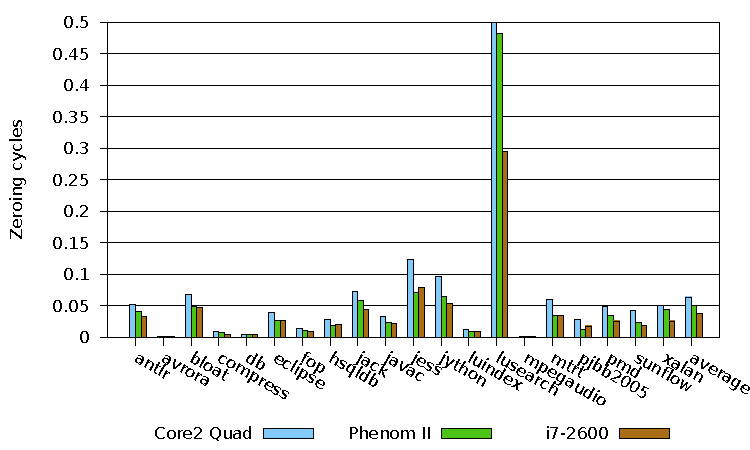
\includegraphics[width=\columnwidth]{figs/zerocost_intel.pdf}}
%  \subfigure[BytesZeroed / BytesBurstTransactionsTransferred\label{fig:zerobus}]{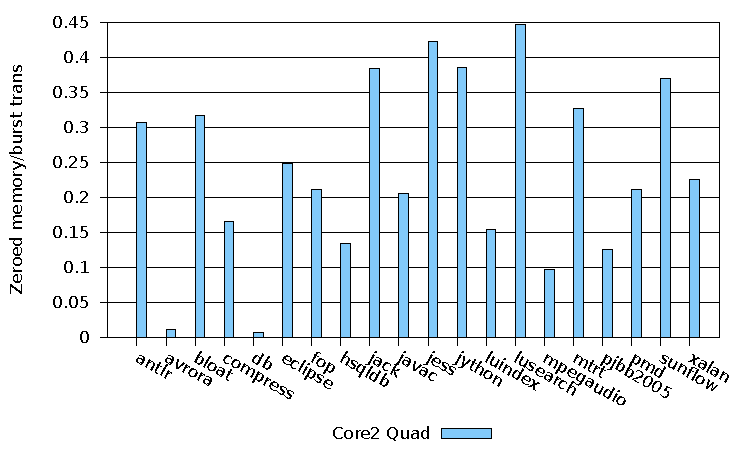
\includegraphics[width=1.0\columnwidth]{figs/zerobus_core.pdf}}
%  \caption{The cost of zero initialization}
%\end{figure*}


%\begin{figure}
%  \centering
%  \subfigure[\label{fig:c:hello}]{
%  \begin{minipage}[b]{\columnwidth}
%    \lstinputlisting[linewidth=\columnwidth,breaklines=true]{code/hello.c}\vspace*{-2ex}
%  \end{minipage}}
%  \subfigure[\label{fig:java:hello}]{
%  \begin{minipage}[b]{\columnwidth}
%    \lstinputlisting[linewidth=\columnwidth,breaklines=true]{code/hello.java}\vspace*{-2ex}
%  \end{minipage}}
%  \caption{Hello world in Java and C.}
%  \label{fig:helloworld}
%\end{figure}

%\section{Summary}

\chapter{Discussion}
\label{cha:discussion}

E

\section{Foreground Removal}
\label{sec:fr_disc}

\begin{itemize}
    \item Edge Detection and Rippling
    \item Comparison of Methods
    \item Sample Size Limitations
\end{itemize}

\subsection{Edge Detection and Rippling}
\label{ssec:A1}

E

\subsection{Comparison of Methods}
\label{ssec:A2}

E

\subsection{Sample Size Limitations}
\label{ssec:A3}

E

\section{Magnetic Field Derivation}
\label{sec:mag_disc}

\begin{itemize}
    \item Data Collection
    \begin{itemize}
        \item HI and H-alpha Data (Not needed!)
    \end{itemize}
    \item Neccesity of Assumptions
    \item Validity of Derivation Methods and VGSR
    \item Uncertainty Analysis
\end{itemize}

\subsection{Data Collection}
\label{ssec:B1}

E

\subsection{Neccesity of Assumptions}
\label{ssec:B2}

E

\subsection{Validity of Derivation Methods}
\label{ssec:B3}

E

\subsection{Uncertainty Analysis}
\label{ssec:B4}

E

\chapter{Conclusions}
\label{cha:conclusion}

E

Also comment on projects in current development. Including \cite{ID70, ID72, ID67}.



%%%%%%%%%%%%%%%%%%%%%%%%%%%%%%%%%%%%%%%%%%%%%%%%%%%%%%%%%%%%%%%%%%%%%%
% Here begins the end matter

\setcounter{chapter}{7}
\setcounter{section}{0}

\renewcommand*{\thechapter}{}

\appendix

\chapter{Appendix}
\label{cha:appendix}

\renewcommand*{\thesection}{\Alph{section}}

\section{Developed code and data}
\label{sec:appendixA}

All developed code and data is found in a publically-available GitHub repository as shown here: \url{https://github.com/Olivex727/hvc-magnetic-honours-programs}.

\section{All HVCs and HVC Calulations}
\label{sec:appendixB}

The filtered Moss catalogue is as below.


\section{Planck Mission Cosmic Microwave Background}
\label{sec:appendixC}

The source for the Planck mission's CMB temperature map is available on this website: \url{https://www.esa.int/ESA_Multimedia/Images/2013/03/Planck_CMB/}.

\section{PyNUFFT Python Module}
\label{sec:appendixD}

The pyNUFFT Python Module, which was used in the investigation for foreground removal, has its main documentation page here: \url{https://pynufft.readthedocs.io/en/latest/index.html}

\section{Statistical ANOVA Tests}
\label{sec:appendixE}

The R language was used to calculate all tests mentioned in \ref{ssec:results_stats}, the file is available here: \url{https://github.com/Olivex727/hvc-magnetic-honours-programs/blob/main/KS_confirmation/wgt_anova.R}.

The specific R code output when running this file is as follows:

\begin{verbatim}
> summary(base_V2_aov)
Df Sum Sq Mean Sq F value Pr(>F)  
data_new$variable.x  2   44.7  22.349   3.375 0.0388 *
Residuals           87  576.1   6.622                 
---
Signif. codes:  0 '***' 0.001 '**' 0.01 '*' 0.05 '.' 0.1 ' ' 1
> tukey.test
Tukey multiple comparisons of means
95% family-wise confidence level

Fit: aov(formula = data_new$Estimate ~ data_new$variable.x,
weights = data_new$prescision)

$`data_new$variable.x`
   diff       lwr         upr     p adj
Var_Sub-KS_EDF   -1.199 -2.783335  0.38533482 0.1741072
Wgt_Mean-KS_EDF  -1.675 -3.259335 -0.09066518 0.0357301
Wgt_Mean-Var_Sub -0.476 -2.060335  1.10833482 0.7544765

> 
\end{verbatim}

A copy of this text output is available in the file: \url{https://github.com/Olivex727/hvc-magnetic-honours-programs/blob/main/KS_confirmation/chisq.txt}.

\backmatter

\bibliographystyle{anuthesis}
\bibliography{thesis, batch1, batch1additional, batch2rand, obstech}

\printindex

\end{document}
